\chapter{Pattern Sequenziali Frequenti}
\label{ch:seq}

Questo capitolo descrive un'analisi effettuata sul solo data set degli studenti. L'idea generale è quella di estrarre dei \textit{pattern sequenziali} dal data set ottenuto nella fase di \textit{preprocessing} descritta nella Sezione \ref{prepr:seq}, per poi analizzarli ulteriormente con degli script Python realizzati \textit{ad hoc}.

\section{Algoritmo GSP}

    Per l'estrazione dei pattern sequenziali \textbf{frequenti} è stato fatto uso dell'algoritmo \textit{Generalized Sequential Pattern}. Una breve descrizione del funzionamento di tale algoritmo può essere trovata in \cite{gsp}: \\

    "There are two main steps in the algorithm:
    \begin{itemize}
        \item \textbf{Candidate Generation}. Given the set of frequent (k-1)-frequent sequences F(k-1), the candidates for the next pass are generated by joining F(k-1) with itself. A pruning phase eliminates any sequence, at least one of whose subsequences is not frequent.
        \item \textbf{Support Counting}. Normally, a hash tree–based search is employed for efficient support counting. Finally non-maximal frequent sequences are removed.
    \end{itemize}

    The algorithms for solving sequence mining problems are mostly based on the \textit{a priori} (level-wise) algorithm." \\

    Parafrasando quanto sopra riportato, l'algoritmo GSP è basato sul \textbf{principio Apriori} --- lo stesso già incontrato in \ref{apriori}, per quanto riguardava la ricerca di regole associative. \\

    L'implementazione utilizzata per l'analisi in oggetto, è quella fornita da Weka. Come si può vedere in Figura \ref{gsp_weka}, si tratta di una versione piuttosto basilare in cui si può specificare un limitato numero di parametri; tuttavia, la (poca) flessibilità concessa è risultata sufficiente al raggiungimento dello scopo.

    \begin{figure}
        \centering
        \caption{finestra che mostra i parametri impostabili dell'implementazione di DBSCAN su Weka}
        \label{gsp_weka}
        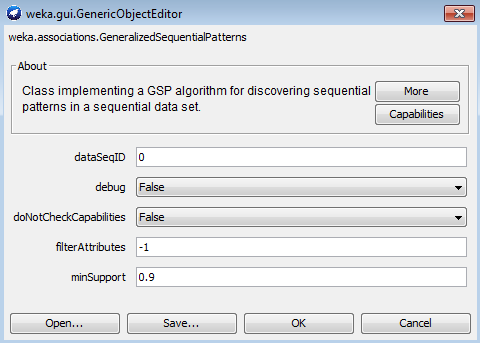
\includegraphics[scale=0.75]{img/gsp.png}
    \end{figure}

\section{Scopo dell'Analisi}

    Questa analisi si basa sull'idea di considerare come \textit{pattern sequenziale} l'ordine in cui ogni studenti ha superato i vari esami del Corso di Laurea, ignorando l'entità del \textit{gap} presente fra il superamento di un esame e l'altro\footnote{Tale elemento, che caratterizza in modo significativo le prestazioni degli studenti, è stato ampiamente considerato nelle analisi descritte negli altri capitoli di questo documento.} e il voto conseguito.\\

    Avendo ben chiara questa astrazione, lo scopo che ci si è prefissati è quello di confrontare le varie sequenze di esami con una \textit{sequenza ideale}. Data la codifica degli esami riportata in Tabella \ref{exams_code}, si è intesa come tale sequenza ideale la seguente: \\

    \begin{centering}
        \texttt{1\_ASD, 1\_ADE, 1\_AN1, 1\_PRG, 1\_MDL, 1\_ENG} \\
        \texttt{2\_1\_ALG, 2\_1\_MDP, 2\_1\_CPS, 2\_1\_PRC} \\
        \texttt{2\_2\_AN2, 2\_2\_FIG, 2\_2\_BDS, 2\_2\_SOP} \\
        \texttt{3\_1\_REC, 3\_1\_INC, 1\_1\_CAZ, 3\_2\_CAN, 3\_2\_ITE} \\
    \end{centering}

    \vspace{0.35cm}

    In pratica, è stato considerato come ordine ideale per superare i corsi quello naturale previsto dal Corso di Laurea, contando come non rilevante la posizione degli esami i cui corsi sono svolti nello stesso periodo --- ad esempio, non si è considerato importante l'ordine in cui sono stati superati gli esami del primo anno, a patto che siano stati intrapresi con successo prima degli esami successivi. \\

    \begin{table}
    \begin{tabular}{ll}
    \hline
    \textbf{Esame}                         & \textbf{Codifica} \\ \hline
    Algoritmi e Strutture Dati             & 1\_ASD            \\
    Architetture degli Elaboratori         & 1\_ADE            \\
    Analisi 1                              & 1\_AN1            \\
    Programmazione                         & 1\_PRG            \\
    Matematica Discreta e Logica           & 1\_MDL            \\
    Inglese                                & 1\_ENG            \\
    Algebra Lineare                        & 2\_1\_ALG         \\
    Metodologie di Programmazione          & 2\_1\_MDP         \\
    Calcolo della Probabilità e Statistica & 2\_1\_CPS         \\
    Programmazione Concorrente             & 2\_1\_PRC         \\
    Analisi 2                              & 2\_2\_AN2         \\
    Fisica Generale                        & 2\_2\_FIG         \\
    Basi di Dati e Sistemi Informativi     & 2\_2\_BDS         \\
    Sistemi Operativi                      & 2\_2\_SOP         \\
    Reti di Calcolatori                    & 3\_1\_REC         \\
    Interpreti e Compilatori               & 3\_1\_INC         \\
    Competenze Aziendali                   & 3\_1\_CAZ         \\
    Calcolo Numerico                       & 3\_2\_CAN         \\
    Informatica Teorica                    & 3\_2\_ITE         \\ \hline
    \end{tabular}
    \caption{Tabella che mostra l'associazione fra il nome di ogni esame e la sua codifica nei pattern sequenziali.}
    \label{exams_code}
    \end{table}

    Una volta ottenute le sequenze di esami che compaiono frequentemente nei dati degli studenti \textit{preprocessati}, lo step successivo consiste nell'individuare in esse gli esami che sono più frequentemente \textbf{fuori posto} rispetto alla seuenza ideale precedentemente descritta. Questo ci consente di ampliare la conoscenza di quanto già compreso negli altri capitolo riguardo a quali sono i corsi che creano più difficoltà agli studenti --- o che comunque, in questo specifico caso, vengono rimandati più spesso in favore di altri esami teoricamente successivi ad essi. \\

    \subsection{Esempio di Analisi di una Sequenza Frequente}

    Si porta un esempio, per assicurarsi una chiarezza totale nell'esposizione di quella che è l'idea fondamentale dell'intera analisi. Si assuma che l'algoritmo GSP restituisca come output il seguente pattern sequenziale frequente: \\

    \begin{centering}
        \texttt{1\_ASD, 1\_PRG, 2\_1\_MDP, 1\_MDL, 2\_1\_PRC}
    \end{centering}

    \vspace{0.35cm}

    Il fatto che la sequenza è frequente, significa ovviamente che quello è "un pezzo" della carriera di molti\footnote{Si utilizza la locuzione \textit{molti} grazie alla sua flessibilità, visto che la quantità di istanze necessarie affinché una sequenza diventi frequente cambia a seconda del supporto inserito come criterio di potatura.} studenti. La caratteristica apparente di tale sequenza di esami è che Matematica Discreta e Logica, un esame del primo anno, è stato superato \textit{dopo} Metodologie di Programmazione, un esame del primo semestre del secondo anno. Questa contraddizione è evidente, se confrontaìiamo questa sequenza con quella ideale: significa che molti studenti hanno deviato da quello che è il percorso pianificato.\\

    Quello che ci si prefigge di fare è, quindi, analizzare in questo senso tutte le sequenze frequenti generate da GSP --- e saranno così tante da rendere impossbile vagliarle tutte come fatto per quella di esempio. Pertanto, come si vedrà, si useranno degli script per automatizzare tale lavro.

\section{Procedimento di Analisi}

    Come si è appena accennato, il vero scopo di ottenere dei pattern sequenziali frequenti non è tanto quello di considerarli come tali --- e si vedrà presto che, in ogni caso, sarebbe impossibile farlo --- ma quello di usarli come base per ulteriori operazioni di \textit{data mining}. \\

    Senza dilungarsi in eccessive descrizioni, si illustra di seguito il procedimento seguito per ottenere i risultati che verranno mostrati nella sezione immediatamente sucessiva alla presente.

    \begin{itemize}
        \item \textbf{Preprocessing dei dati grezzi sugli studenti}: si veda quanto già descritto nella Sezione \ref{prepr:seq}.
        \item \textbf{Lancio dell'algoritmo GSP}: si tratta del passo fondamentale di tutto il processo, in quanto consente di ottenere i pattern sequenziali frequenti su cui poi lavorare ulteriormente. Come si vedrà in seguito, in questa fase è stato riscontrato il primo, vero problema di \textit{big data} dell'intero lavoro svolto per questa tesi.
        \item \textbf{\textit{Mining} di pattern inusuali}: gli output prodotti dall'algoritmo GSP vengono analizzati e filtrati, in modo da considerare soltanto i pattern che presentano un'anomalia rispetto alla sequenza di esami ideale. Questo viene realizzato tramite lo script Python riportato in \ref{appendix:unusual}.
        \item \textbf{\textit{Mining} degli esami "fuori posto"}: si analizza ulteriormente l'output del precedente step, andando a creare una sintesi di quali particolari esami hanno causato l'anomalia delle sequenze trovate. Tale scopo è stato raggiunto grazie allo script Python riportato in \ref{appendix:freq}.
    \end{itemize}

    \subsection{Lancio di GSP}

        Gli output restituiti da GSP sono di questa forma: \\

        \begin{lstlisting}
            GeneralizedSequentialPatterns
            =============================

            Number of cycles performed: 7
            Total number of frequent sequences: 19478

            Frequent Sequences Details (filtered):
            
            - 1-sequences
            [1] <{1_ASD}> (147)
            [2] <{1_ADE}> (137)
                - omiss. -

            - 2-sequences

            [1] <{1_ASD}{1_ADE}> (121)
            [2] <{1_ASD}{1_AN1}> (94)
                - omiss. -

            - omiss. -
        \end{lstlisting}

        Per ogni data set preparato precedentemente, l'algoritmo GSP è stato lanciato tre volte, con tre valori diversi di supporto minimo: $0.33$, $0.50$ e $0.75$; in un caso è stato addirittura tentato il lancio con supporto minimo pari a $0.10$. Questo ha prodotto una elevata mole di sequenze frequenti, che è stata appositamente memorizzata in file di testo (Figura \ref{files}), pronti per essere analizzati dai successivi script. \\

        \begin{figure}
            \centering
            \caption{File contenenti i risultati di tutti i lanci dell'algoritmo GSP}
            \label{files}
            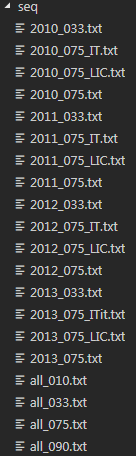
\includegraphics[scale=0.75]{img/seq_files.png}
        \end{figure}

        Come già accennato, la complessità dell'algoritmo GSP ha creato il primo, vero problema relativo all'impiego di \textit{big data}: i tempi di anallisi sulla versione intera del data set preprocessato --- quella che contiene le sequenze di tutte le istanze di studenti a disposizione --- esulano dalla trattabilità. Perciò, per ogni data set preparato, è stato applicato il filtro relativo alla lunghezza della sequenza, scartando tutti gli studenti che non hanno completato almeno un terzo del Corso di Laurea, come già descritto in Sezione ottenuta in Sezione \ref{prepr:seq}. Nonostante questo filtro, i tempi macchina sono stati comunque molto alti per quanto riguarda il data set completo. Per gli altri, invece, si è trattato di computazioni brevi. \\

    \subsection{Filtraggio delle Sequenze Inusuali}

    ...

    \subsection{Sommario degli Esami Non Congruenti}

    ...

\section{Risultati Finali dell'Analisi}

    Si arriva infine a quello che, abbandonandoci alla suggestiva metafora principale del \textit{data mining}, è il vero oro finalmente estratto dall'intera mole di dati della produttività degli studenti:

    ... immagine